%\title{LaTeX Portrait Poster Template}
%%%%%%%%%%%%%%%%%%%%%%%%%%%%%%%%%%%%%%%%%
% a0poster Portrait Poster
% LaTeX Template
% Version 1.0 (22/06/13)
%
% The a0poster class was created by:
% Gerlinde Kettl and Matthias Weiser (tex@kettl.de)
% 
% Adapter by Jens Buysse for Hogeschool Gent
% This template has been downloaded from:
% http://www.LaTeXTemplates.com
%
% License:
% CC BY-NC-SA 3.0 (http://creativecommons.org/licenses/by-nc-sa/3.0/)
%
%%%%%%%%%%%%%%%%%%%%%%%%%%%%%%%%%%%%%%%%%

%----------------------------------------------------------------------------------------
%	PACKAGES AND OTHER DOCUMENT CONFIGURATIONS
%----------------------------------------------------------------------------------------

\documentclass[a0,portrait]{a0poster}

\usepackage{multicol} % This is so we can have multiple columns of text side-by-side
\columnsep=100pt % This is the amount of white space between the columns in the poster
\columnseprule=3pt % This is the thickness of the black line between the columns in the poster

\usepackage[svgnames]{xcolor} % Specify colors by their 'svgnames', for a full list of all colors available see here: http://www.latextemplates.com/svgnames-colors

\usepackage{times} % Use the times font
%\usepackage{palatino} % Uncomment to use the Palatino font

\usepackage{graphicx} % Required for including images
\graphicspath{{figures/}} % Location of the graphics files
\usepackage{booktabs} % Top and bottom rules for table
\usepackage[font=small,labelfont=bf]{caption} % Required for specifying captions to tables and figures
\usepackage{amsfonts, amsmath, amsthm, amssymb} % For math fonts, symbols and environments
\usepackage{wrapfig} % Allows wrapping text around tables and figures
\usepackage[export]{adjustbox}
\usepackage{subfig}

\begin{document}

%----------------------------------------------------------------------------------------
%	POSTER HEADER 
%----------------------------------------------------------------------------------------

% The header is divided into two boxes:
% The first is 75% wide and houses the title, subtitle, names, university/organization and contact information
% The second is 25% wide and houses a logo for your university/organization or a photo of you
% The widths of these boxes can be easily edited to accommodate your content as you see fit

\begin{minipage}[t]{0.75\linewidth}
\VeryHuge \color{HoGentAccent1} \textbf{Kotlin Multiplatform Mobile als alternatief voor native applicaties} \color{Black}\\ % Title
\Huge\textit{een vergelijkende studie en proof-of-concept}\\[2.4cm] % Subtitle
\huge \textbf{Ziggy Moens, Kenneth Saey, Ludwig Stroobant}\\[0.5cm] % Author(s)
\huge Hogeschool Gent, Valentin Vaerwyckweg 1, 9000 Gent\\[0.4cm] % University/organization
\Large \texttt{ziggy.moens@hogent.be} \\
\end{minipage}
%
\begin{minipage}[t]{0.25\linewidth}

\includegraphics[width=13cm,right]{figures/HOGENT_Logo_Pos_rgb.png} 

\end{minipage}

\vspace{1cm} % A bit of extra whitespace between the header and poster content

%----------------------------------------------------------------------------------------

\begin{multicols}{2} % This is how many columns your poster will be broken into, a portrait poster is generally split into 2 columns

%----------------------------------------------------------------------------------------
%	ABSTRACT
%----------------------------------------------------------------------------------------

\color{HoGentAccent1} % Navy color for the abstract

\begin{abstract}
Kotlin Multiplatform Mobile, de nieuwste software development kit van JetBrains, toont momenteel een geschikt alternatief te zijn voor native applicatie ontwikkeling. Zaken die in het voordeel van Kotlin Multiplatform Mobile zijn onder andere snelheid, performantie en ontwikkelsnelheid.
\end{abstract}
%----------------------------------------------------------------------------------------
%	INTRODUCTION
%----------------------------------------------------------------------------------------

\color{HoGentAccent1} 
\section*{Introductie}
\color{black}
\color{black}

Binnen deze bachelorproef wordt nagegaan of Kotlin Multiplatform Mobile een alternatief kan bieden voor native applicatieontwikkeling. Cross-platform ontwikkeling lijkt de laatste tijd steeds interessanter gezien de doorgaans lagere kosten en snellere ontwikkeltijden. 
%----------------------------------------------------------------------------------------
%	GEOLOGY
%----------------------------------------------------------------------------------------

\color{Black} % DarkSlateGray color for the rest of the content
\color{HoGentAccent1} 
\section*{Experimenten}
\color{black}
 In deze studie worden gebruikt gemaakt van volgende applicaties:
 \begin{itemize}
     \item Native Android applicatie
     \item Native iOS applicatie
     \item Kotlin Multiplatform Mobile applicatie met ondersteuning voor Android en iOS
 \end{itemize}
Deze applicaties waren vooral gefocust op het vergelijken van de core van de applicaties, hierdoor hadden deze echter niet veel inhoud. Met deze applicaties werden de verschillen en gelijkenissen opgemeten tussen de native en cross-platform applicaties. Hiervoor werden volgende testcriteria gebruikt: het aantal lijnen code, kostprijs, ontwikkeltijd, compileertijd en de voetafdruk.

\begin{center}
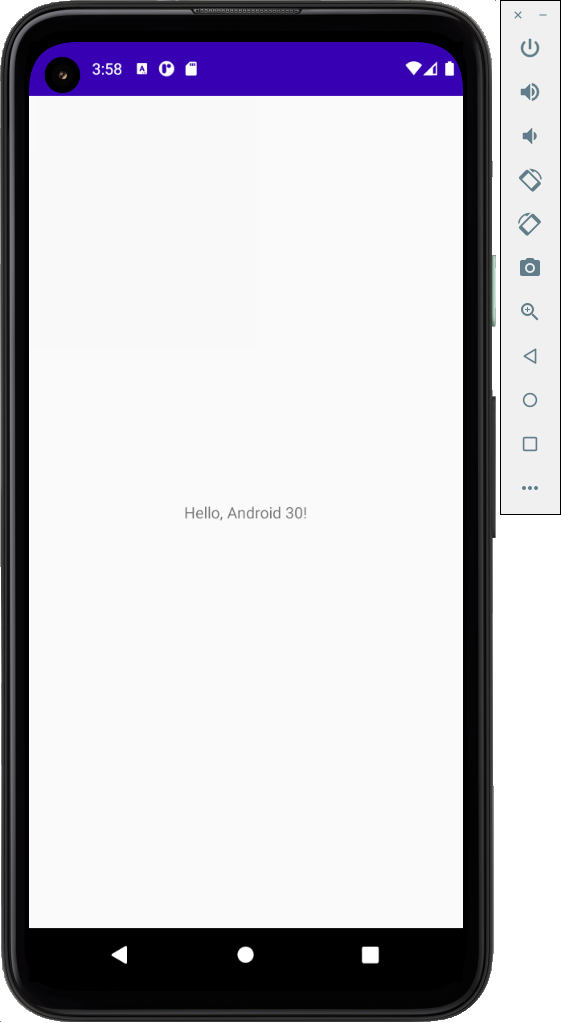
\includegraphics[width=0.45\linewidth]{kmm-basic-android}
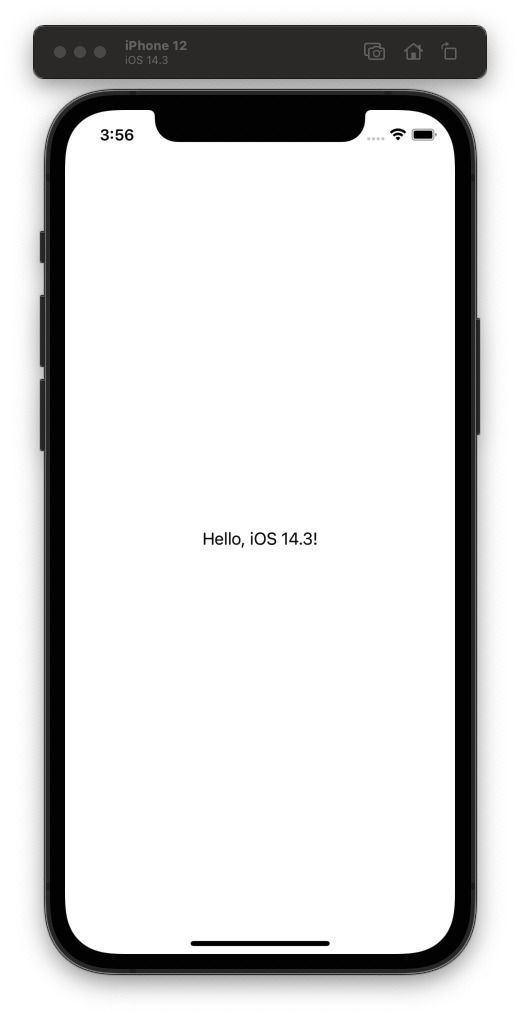
\includegraphics[width=0.45\linewidth]{kmm-basic-ios}
\end{center}



\color{HoGentAccent1} 
\section*{Resulaten}
\color{black}
Uit deze resultaten is gebleken dat Kotlin Multiplatform Mobile veel potentieel toont als alternatief voor native applicaties. Bij het evalueren van deze resultaten dient wel het feit dat Kotlin Multiplatform Mobile zich nog altijd in het alfa stadium bevindt, in het achterhoofd gehouden te worden. Volgende testen speelden in het voordeel van Kotlin Multiplatform Mobile: het aantal lijnen code en de eerste compilatie. Daarnaast waren de native applicaties iets performanter op vlak van voetafdruk.
\\ \\
De testcriteria die de ontwikkelingstijd en de kostprijs evalueerden toonden een klein voordeel voor Kotlin Multiplatform Mobile. Aangezien Kotlin Multiplatform Mobile net sneller te ontwikkelen was kwam deze dus ook als goedkoopste naar boven. Eens de projectmanagementkosten werden ingecalculeerd, was het verschil groter in het voordeel van Kotlin Multiplatform Mobile.

\begin{center}
    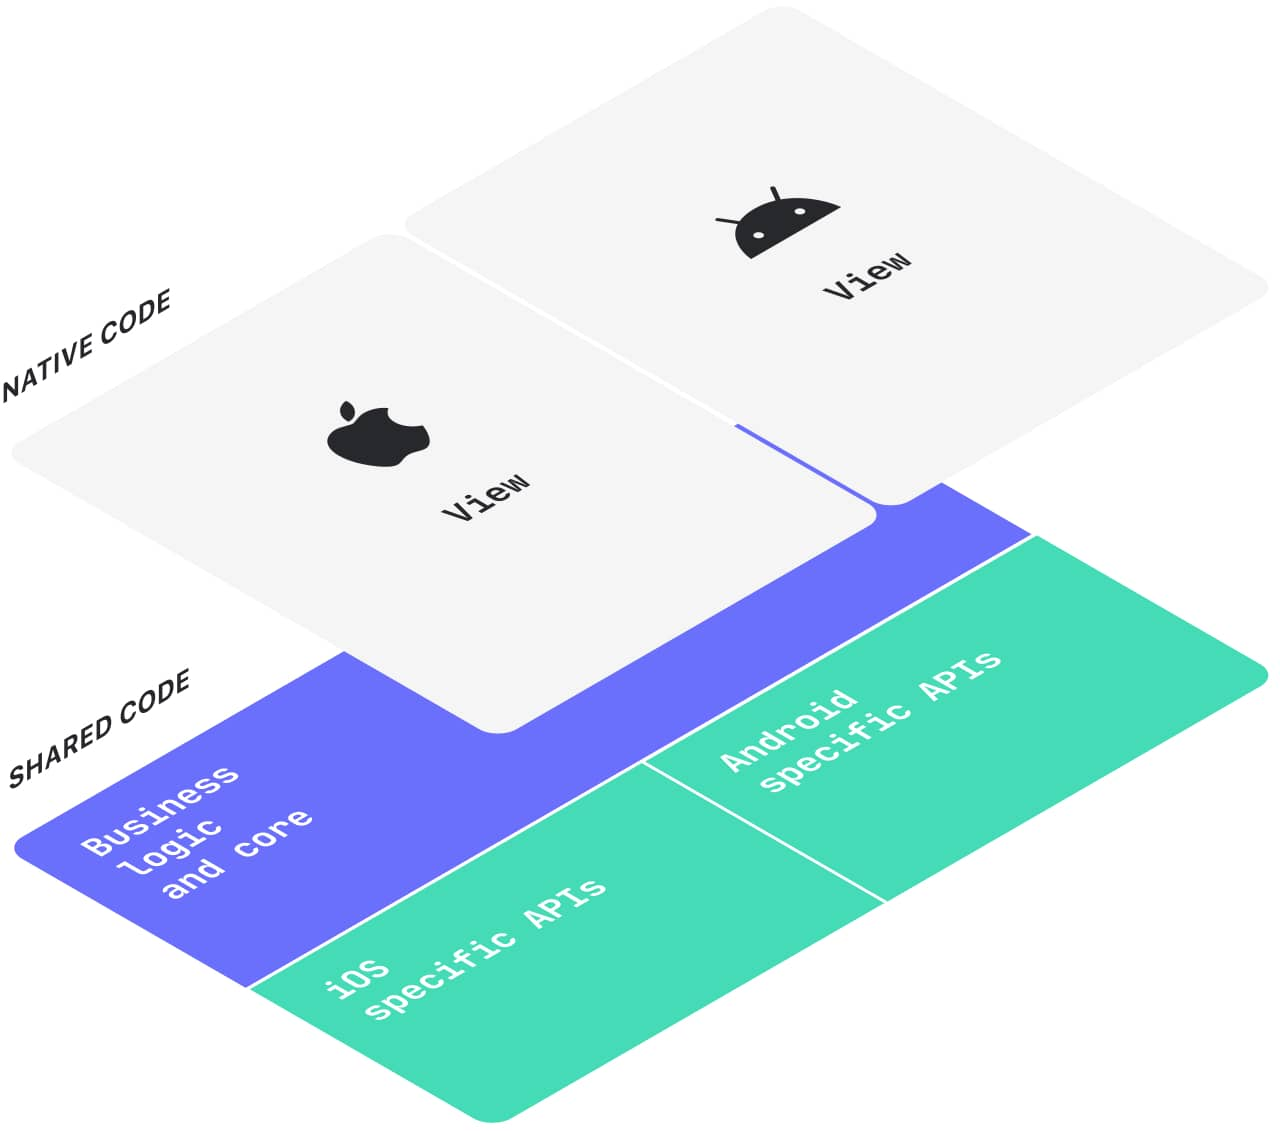
\includegraphics[width=1.0\linewidth]{kmm}
    \captionof{figure}{Grafische voorstelling Kotlin Multiplatform Mobile, https://kotlinlang.org/lp/mobile}
\end{center}

%------------------------------------------------



\color{HoGentAccent1} 
\section*{Conclusies}
\color{black}
Uiteindelijk kenden de cross-platform applicaties dezelfde look en feel als de native applicaties en hadden ongeveer gelijke of zelfs betere resultaten op vlak van snelheid, performantie en ontwikkelingstijd. Dit maakt dat Kotlin Multiplatform Mobile een interessant alternatief kan zijn voor native applicatieontwikkeling. Eens Kotlin Multiplatform Mobile in productie gaat en bedrijven maken de overstap, wordt verondersteld dat Kotlin Multiplatform Mobile hier zeker een voordeel kan bieden.
%----------------------------------------------------------------------------------------
%	FORTHCOMING RESEARCH
%----------------------------------------------------------------------------------------
\color{HoGentAccent1} 
\section*{Toekomstig onderzoek}
\color{black}

Volgend op deze studie zijn er enkele zaken die verder kunnen onderzocht worden, hieronder enkele mogelijke onderzoeksvragen.
\begin{itemize}
    \item Voor de test in verband met de voetafdruk zou een uitgebreidere studie kunnen uitgevoerd worden die meerdere applicaties maakt over een langere periode. Op deze manier zou de voetafdruk van native ten opzichte van KMM beter in kaart kunnen gebracht worden.
    \item De huidige applicatie kan verder uitgebreid worden, aangezien dit een zeer ruim gegeven is, worden al enkele mogelijke uitbreidingen gegeven.
        \begin{itemize}
            \item Toevoegen van tekstvelden en user interface elementen
            \item Off-line data en de verwerking ervan
            \item On-line data aan de hand van API-calls
            \item Toevoegen van wiskundige berekeningen
        \end{itemize}
    Daarnaast kan uitbreiding ook gezien worden als het uitbreiden naar meerdere devices zoals Apple Watch\footnote{apple.com/benl/watch}, iPad\footnote{apple.com/benl/ipad}, Android Auto\footnote{android.com/auto}...
    \item Herhaling van het huidig onderzoek door developers met verschillende graden van
    ervaring binnen het ontwikkelen met Kotlin, Swift en KMM. Aan de hand van deze test zou de impact van de developer op de testresultaten kunnen in kaart gebracht worden.
    \item Kotlin Multiplatform Mobile vergelijken met andere cross-platform frameworks zoals Flutter\footnote{flutter.dev} en React Native\footnote{reactnative.dev}. Aan de hand van deze test zal bepaald kunnen worden of KMM de meest interessante variant is tussen alle cross-platform oplossingen.
\end{itemize}


%----------------------------------------------------------------------------------------

\end{multicols}
\end{document}